\section{Herramienta kt}

\subsection{¿Qu\'e es?}
Supongamos que queremos seguir la estructura de un proyecto de PyQt5 sugerida por esta gu\'ia, \nameref{estructura_programas}, porque resulta pr\'actico
para el manejo de muchos archivos y cuando nos acostumbramos es agradable visualmente. Luego, cada vez que agregamos un Widget, al haberlo creado en QtDesigner debemos
guardarlos en la carpeta designer, y adem\'as compilarlo junto con sus recursos. Y finalmente guardar los resultados de la compilaci\'on en sus respectivas carpetas.
Tambi\'en tenemos que repetir el proceso cada vez que actualizamos o cambiamos algo, esto puede ser un poco tedioso.

Para resolver estos inconvenientes, sub\'i un script para automatizar estos procesos, de forma muy sencilla.

\subsection{Instalaci\'on}
El proceso de instalaci\'on consiste en clonar el repositorio, o simplemente en alg\'un lado de nuestro sistema guardar el script "kt.py", luego
agregarlo a las variables de entorno del sistema operativo para usarlo desde cualquier lado.

\begin{itemize}
    \item 1. Clonamos el repositorio de GitHub.
    \item 2. Agregamos a las variables de entorno la direcci\'on a la carpeta /tools dentro del repositorio. En \nameref{error_de_consola}, se explica como agregar esa variable, pero con Python.
    \item 3. Listo!
\end{itemize}

\subsection{Uso}

\subsubsection{Creaci\'on de un proyecto}
Cuando queremos crear un proyecto, es decir, crear la estructura del directorio correspondiente a lo convenido por la gu\'ia,
debemos ir a la carpeta principal del proyecto, y ejecuta la siguiente l\'inea. El uso del nombre de la aplicaci\'on est\'a sujeto a la versi\'on
de la herramienta, en su creaci\'on no era usado pero se dej\'o por futuras funcionalidades.

\begin{center}
    \textbf{kt.py app NombreDeAplicaci\'on}
\end{center}

\begin{figure}[H]
    \centering
    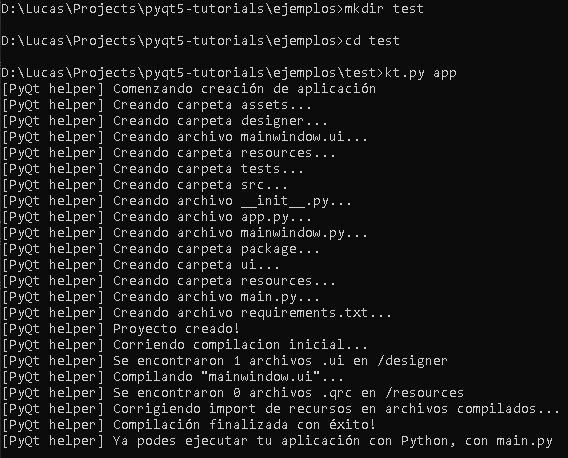
\includegraphics[width=0.9\linewidth]{imagenes/kt/app.png}
    \caption{Creaci\'on de proyecto con herramiento kt}
    \label{fig:creacion_app_kt}
\end{figure}

\subsubsection{Compilaci\'on de .ui y .qrc}
La compilaci\'on de los archivos .ui y .qrc antes era tediosa, ten\'iamos que compilar uno por uno, luego deb\'iamos
corregir un bug del QtDesigner, que al compilar importaba mal los recursos. Y luego mover correctamente a las carpetas de la estructura convenida,
pero ya no m\'as. En la carpeta del proyecto, debemos ejecutar,

\begin{center}
    \textbf{kt.py compile}
\end{center}

\begin{figure}[H]
    \centering
    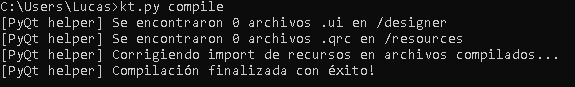
\includegraphics[width=0.9\linewidth]{imagenes/kt/compile.png}
    \caption{Compilaci\'on de proyecto con herramiento kt}
    \label{fig:compilacion_kt}
\end{figure}

\begin{figure}[H]
    \centering
    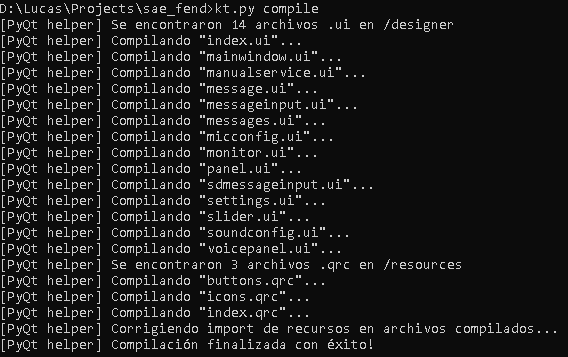
\includegraphics[width=0.9\linewidth]{imagenes/kt/muestra.png}
    \caption{Compilaci\'on de proyecto real con herramienta kt}
    \label{fig:muestra_compilacion_kt}
\end{figure}